%%%%%%%%%%%%%%%%%%%%%%%%%%%%%%%%%%%%%%%%%%%%%%%%%%%%%%%
%                File: OpEx_temp.tex                  %
%                  Date: Sept. 2, 2009                %
%                                                     %
%           LaTeX template file for use with          %
%           OSA's journal Optics Express              %
%                                                     %
%  send comments to Jennifer Mayfield, jmayfi@osa.org %
%                                                     %
% This file requires style file, opex3.sty, under     %
%              the LaTeX article class                %
%                                                     %
%   \documentclass[10pt,letterpaper]{article}         %
%   \usepackage{opex3}                                %
%                                                     %
% Note that our online submission system does not     %
% currently process PDFLaTeX; if PDFLaTeX must be     %
% used, pls. contact OpEx staff, and we will process  %
% manually                                            %
%                                                     %
%                                                     %
%       (c) 2009 Optical Society of America           %
%%%%%%%%%%%%%%%%%%%%%%%%%%%%%%%%%%%%%%%%%%%%%%%%%%%%%%%

%%%%%%%%%%%%%%%%%%%%%%% preamble %%%%%%%%%%%%%%%%%%%%%%%%%%%
\documentclass[10pt,letterpaper]{article}
\usepackage{opex3}

 %\usepackage{ae} %%for Computer Modern fonts

%%%%%%%%%%%%%%%%%%%%%%% begin %%%%%%%%%%%%%%%%%%%%%%%%%%%%%%
\begin{document}

%%%%%%%%%%%%%%%%%% title page information %%%%%%%%%%%%%%%%%%
\title{Simple template for authors submitting to \textit{Optics Express}}

\author{M. Scott Dineen and Jennifer Mayfield}

\address{Optics Express Office, Publications Department, Optical Society of America, \\ Washington, D.C., 20036}

\email{opex@osa.org} %% email address is required

% \homepage{http:...} %% author's URL, if desired

%%%%%%%%%%%%%%%%%%% abstract and OCIS codes %%%%%%%%%%%%%%%%
%% [use \begin{abstract*}...\end{abstract*} if exempt from copyright]

\begin{abstract}
A simple template with some examples is provided for preparing \textit{Optics Express} manuscripts in \LaTeX. For complete instructions, see \texttt{OpEx\_style.tex}. Note that the style file \texttt{opex3.sty} replaces \texttt{opex2.sty}. Additional information on style and submissions is available at \mbox{\url{http://www.opticsexpress.org/submission}}.
\end{abstract}

\ocis{(000.0000) General.} % REPLACE WITH CORRECT OCIS CODES FOR YOUR ARTICLE

%%%%%%%%%%%%%%%%%%%%%%% References %%%%%%%%%%%%%%%%%%%%%%%%%
\begin{thebibliography}{99}

\bibitem{gallo99} K. Gallo and G. Assanto, ``All-optical diode based on second-harmonic generation in an asymmetric waveguide,'' \josab {\bf 16,} 267--269 (1999).

\end{thebibliography}

%%%%%%%%%%%%%%%%%%%%%%%%%%  body  %%%%%%%%%%%%%%%%%%%%%%%%%%
\section{Introduction}

Standard \LaTeX{} or AMS\TeX{} environments should be used to place tables, figures, and math. Examples are given below.

\begin{verbatim}
\begin{figure}[htbp]
%\centering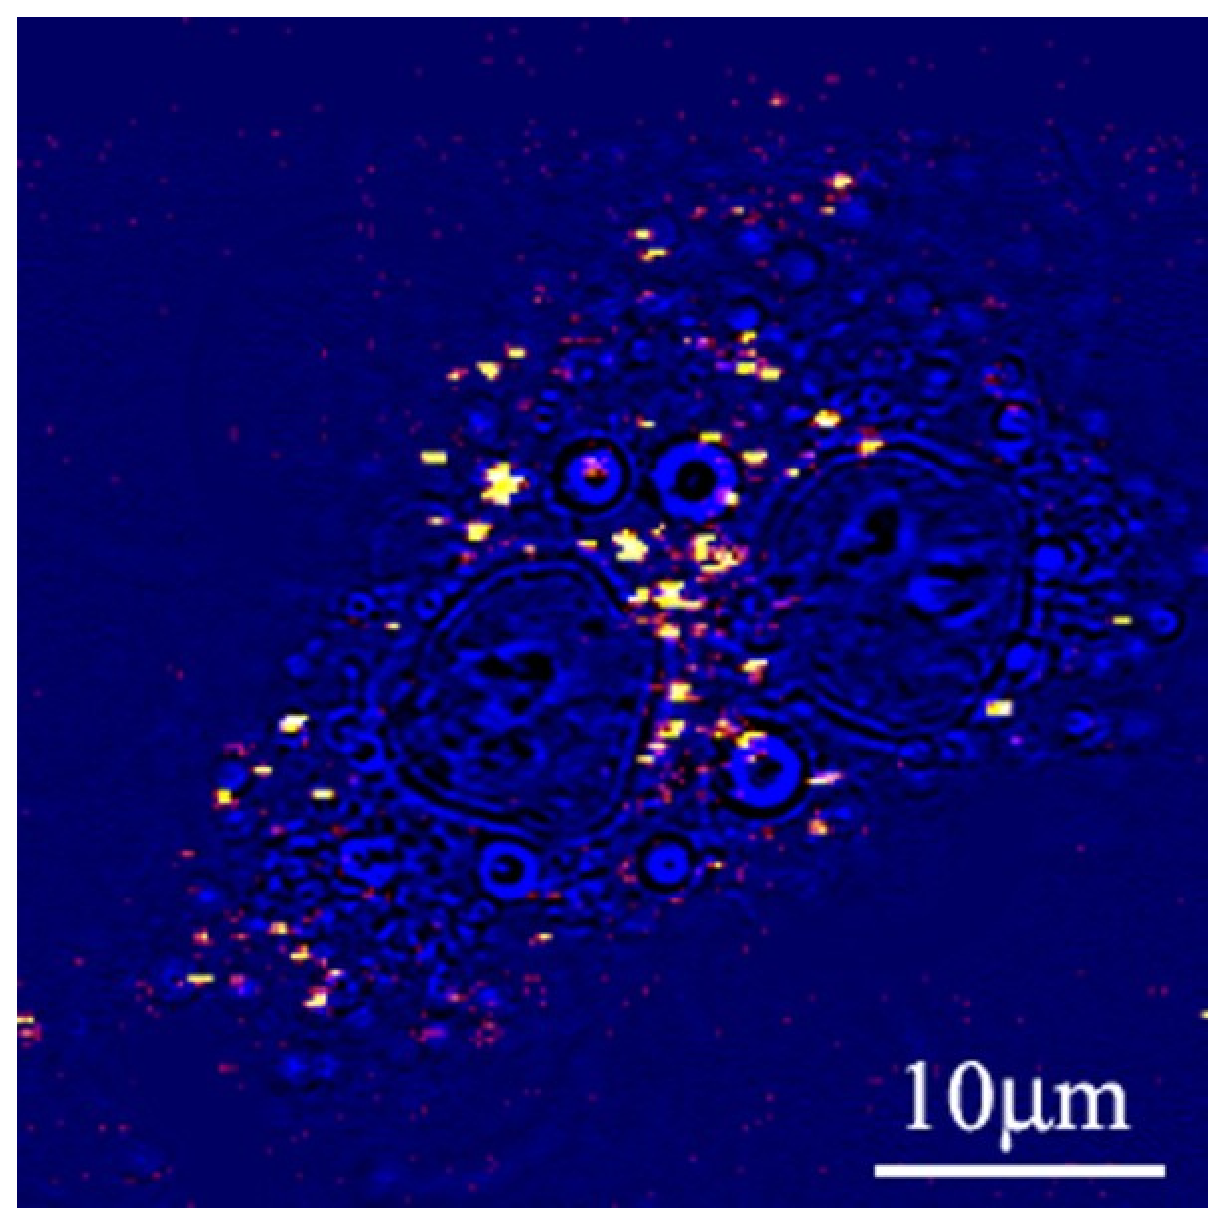
\includegraphics[width=7cm]{opexfig1}
\caption{Sample caption (Ref. \cite{Oron03}, Fig. 2).}
\end{figure}

\begin{equation}
H = \frac{1}{2m}(p_x^2 + p_y^2) + \frac{1}{2} M{\Omega}^2
     (x^2 + y^2) + \omega (x p_y - y p_x).
\end{equation}
\end{verbatim}

\section{Conclusion}
After proofreading the manuscript, tar and gzip the \texttt{.tex} file and
figures; then enter the requested information into the \textit{Optics Express}
online submission system at \url{http://www.opticsexpress.org} and upload the tarred and gzipped archive. If there is video or other multimedia, the associated
files should be uploaded separately.

\end{document} 
